\documentclass[11pt,a4paper]{article}

% ===================== PRÉAMBULE =====================
\usepackage[french]{babel}
\usepackage[utf8]{inputenc}
\usepackage[T1]{fontenc}
\usepackage[a4paper,top=2.5cm,bottom=2.5cm,left=2.5cm,right=2.5cm]{geometry}
\usepackage{graphicx}
\usepackage{booktabs}
\usepackage{array}
\usepackage{longtable}
\usepackage{amsmath}
\usepackage{amssymb}
\usepackage{xcolor}
\usepackage{colortbl}
\usepackage{enumitem}
\usepackage{fancyhdr}
\usepackage{titlesec}
\usepackage[hidelinks]{hyperref}
\usepackage{caption}
\usepackage[expansion=false]{microtype}
\usepackage{parskip}

% ----- Couleurs EMSI -----

% ----- En-têtes / pieds de page -----
\pagestyle{fancy}
\fancyhf{}
\renewcommand{\headrulewidth}{0.4pt}
\fancyhead[L]{\small EMSI Casablanca --- Projet de fin de module Deep Learning --- 2025--2026}
\fancyfoot[C]{\thepage}

% ----- Style des titres -----
\titleformat{\section}{\Large\bfseries}{\thesection}{1em}{}
\titleformat{\subsection}{\large\bfseries}{\thesubsection}{1em}{}
\titleformat{\subsubsection}{\normalsize\bfseries}{\thesubsubsection}{1em}{}

% ----- Légendes de figures/tableaux -----
\captionsetup{labelfont=bf,font=small,margin=1cm}

\newcommand{\python}[1]{\texttt{#1}}

% ===================== DOCUMENT =====================
\begin{document}

% --------------------- PAGE DE GARDE ---------------------
\begin{titlepage}
\centering
\vspace*{1cm}

{\Large\bfseries EMSI Casablanca}\\[0.3cm]
{\large École Marocaine des Sciences de l'Ingénieur}\\[0.2cm]
{\large Filière Informatique}\\[0.2cm]
{\large Module : Deep Learning --- Année universitaire 2025--2026}

\vspace{2.5cm}
\rule{0.8\textwidth}{0.6pt}\\[0.6cm]
{\huge\bfseries PROJET DE FIN DE MODULE}\\[1cm]
{\Large\bfseries Conception, implémentation, comparaison et analyse critique de modèles de deep learning pour données tabulaires, images et séquences}\\[0.8cm]
\rule{0.8\textwidth}{0.6pt}

\vspace{1cm}
{\large\itshape Travail individuel --- Examen final intégrateur}

\vspace{3cm}

\begin{flushleft}
\large
\textbf{Nom de l'étudiant(e)~:} \makebox[8cm]{\hrulefill}\\[0.8cm]
\textbf{Encadrant(e)~:} \makebox[8cm]{\hrulefill}\\[0.8cm]
\textbf{Date~:} Juin 2026
\end{flushleft}

\vfill
\end{titlepage}

% --------------------- SOMMAIRE ---------------------
\tableofcontents
\bigskip
\noindent\textit{(Sommaire généré automatiquement par LaTeX --- recompiler le document pour le mettre à jour.)}

\newpage

% ===================== INTRODUCTION GÉNÉRALE =====================
\section*{Introduction générale}
\addcontentsline{toc}{section}{Introduction générale}

Le deep learning ne propose pas une architecture unique capable de traiter indifféremment tout type de données~: il propose au contraire une famille de paradigmes dont chacun encode, dans sa structure même, une hypothèse sur la nature des données qu'il traite. Un perceptron multicouche (MLP) suppose des variables d'entrée indépendantes et permutables~; un réseau convolutionnel (CNN) suppose une structure spatiale locale et une invariance par translation~; un réseau récurrent (RNN, LSTM, GRU) suppose une dépendance séquentielle et temporelle entre les observations. Le présent projet a pour objectif de mettre en évidence, par la théorie autant que par l'expérimentation, l'adéquation entre la structure d'une architecture et la géométrie des données qu'elle est appelée à traiter.

Ce rapport constitue la restitution du projet de fin de module de Deep Learning de l'EMSI Casablanca. Conformément aux consignes, il couvre de façon indépendante mais cohérente les trois grandes familles de modèles étudiées durant le module~: le perceptron multicouche appliqué à des données tabulaires, le réseau convolutionnel appliqué à des données image, et les architectures récurrentes (RNN, LSTM, GRU, Seq2Seq) appliquées à des données séquentielles textuelles. Chaque partie suit la même trame~: une étude théorique des concepts mobilisés, une description de la méthodologie et des données, une implémentation sous PyTorch, une étude expérimentale comparative, une interprétation critique des résultats, et une réponse argumentée à la question de synthèse posée dans le sujet.

\subsection*{Choix des jeux de données}
\addcontentsline{toc}{subsection}{Choix des jeux de données}

Le sujet autorise explicitement le recours à « tout autre dataset équivalent validé par l'enseignant(e) ». L'environnement d'exécution utilisé pour ce projet ne disposant pas d'un accès réseau général (les téléchargements sont restreints à quelques dépôts de paquets logiciels), les trois jeux de données ont été choisis parmi ceux qui sont soit directement intégrés aux bibliothèques scientifiques utilisées, soit composés manuellement, tout en conservant la même nature statistique que les jeux de référence suggérés par le sujet~:

\begin{itemize}[leftmargin=1.2cm]
\item \textbf{Partie I (tabulaire)}~: Breast Cancer Wisconsin (569 observations, 30 variables, classification binaire), intégré à scikit-learn --- il s'agit précisément du second exemple proposé par le sujet.
\item \textbf{Partie II (image)}~: UCI Digits (1797 images réelles de chiffres manuscrits, 8$\times$8 pixels en niveaux de gris, 10 classes), intégré à scikit-learn --- un analogue plus compact de MNIST, partageant sa nature (chiffres manuscrits) et sa problématique (classification d'images en niveaux de gris).
\item \textbf{Partie III (séquentiel)}~: un corpus parallèle anglais--français de 68 paires de phrases composé manuellement, dans l'esprit d'un sous-ensemble simplifié de type Tatoeba/fra-eng, option explicitement proposée par le sujet.
\end{itemize}

Cette substitution ne modifie en rien la méthodologie attendue~: les mêmes opérations (nettoyage, normalisation, séparation des ensembles, choix d'architecture, étude d'ablation, métriques d'évaluation) sont appliquées à l'identique. Toutes les expériences présentées dans ce rapport ont été réellement exécutées~; les résultats chiffrés, figures et exemples de traduction reproduits ci-après sont donc des résultats authentiques et non des valeurs illustratives, à l'exception de la conclusion stylistique demandée qui invite à considérer ces résultats comme représentatifs de la méthode plutôt que comme une performance définitive --- un jeu de données plus volumineux (MNIST complet, corpus Tatoeba complet) renforcerait la significativité statistique des écarts observés sans changer la nature des conclusions méthodologiques.

\subsection*{Organisation du rapport}
\addcontentsline{toc}{subsection}{Organisation du rapport}

Le rapport est structuré en trois parties principales correspondant aux trois familles de modèles, suivies d'une synthèse transversale répondant à la problématique générale du projet, d'une conclusion générale, d'une bibliographie indicative et d'une annexe expérimentale regroupant les tableaux récapitulatifs et les éléments complémentaires. Le code source complet, commenté et exécutable, ainsi que le notebook Jupyter associé, sont livrés séparément de ce document.

\newpage
% ===================== PARTIE I =====================
\section{Partie I --- MLP et ingénierie PyTorch}

\textit{Thème~: classification supervisée sur données tabulaires réelles à l'aide d'un perceptron multicouche (MLP). Dataset retenu~: Breast Cancer Wisconsin (569 observations, 30 variables numériques décrivant des caractéristiques de noyaux cellulaires, 2 classes~: tumeur maligne / bénigne).}

\subsection{Fondements théoriques}

Un MLP est une composition de transformations affines et de non-linéarités. Sous PyTorch, toute couche ou tout modèle hérite de la classe \texttt{nn.Module}, qui assure trois fonctions essentielles~: l'enregistrement automatique des paramètres apprenables (poids et biais) dans un graphe d'attributs, la mise à disposition de la méthode \texttt{forward()} qui définit la propagation avant, et la construction implicite, lors de cet appel, du graphe de calcul utilisé par \texttt{autograd} pour la rétropropagation. Chaque paramètre est un tenseur muni de l'attribut \texttt{requires\_grad=True}~; lors de l'appel à \texttt{loss.backward()}, PyTorch parcourt le graphe en sens inverse et accumule, dans l'attribut \texttt{.grad} de chaque paramètre, la dérivée partielle de la fonction de perte par rapport à ce paramètre, via la règle de dérivation en chaîne. L'optimiseur (ici Adam) utilise ensuite ces gradients pour mettre à jour les paramètres.

La méthode \texttt{state\_dict()} renvoie un dictionnaire ordonné associant à chaque paramètre (et, le cas échéant, à chaque statistique de couches comme BatchNorm) son nom et sa valeur courante~; c'est cette structure qui est sérialisée lors d'une sauvegarde et qui permet de recharger un modèle de même architecture. La méthode \texttt{named\_parameters()} fournit un itérateur similaire mais orienté vers l'inspection (forme, exigibilité du gradient) plutôt que vers la persistance. Enfin, la notion de \emph{device} désigne le support matériel (CPU ou GPU/CUDA) sur lequel résident à la fois les tenseurs de données et les paramètres du modèle~: ces deux ensembles de tenseurs doivent impérativement résider sur le même device, sous peine d'erreur d'exécution, ce qui justifie l'appel explicite à \texttt{.to(device)} sur le modèle et sur chaque lot de données.

\subsection{Préparation des données}

Le jeu de données Breast Cancer Wisconsin ne comporte pas de valeurs manquantes ni de variables catégorielles à encoder~: les 30 variables sont toutes numériques continues (rayon, texture, périmètre, aire, etc., calculées à partir d'images de cytologie). La variable cible est binaire (0 = tumeur maligne, 1 = tumeur bénigne). La préparation a néanmoins nécessité les étapes suivantes, essentielles pour un MLP entraîné par descente de gradient~:

\begin{itemize}[leftmargin=1.2cm]
\item Séparation stratifiée en trois ensembles disjoints~: 70~\% apprentissage (398 observations), 15~\% validation (85 observations) et 15~\% test (86 observations), la stratification garantissant une proportion comparable des deux classes dans chaque sous-ensemble.
\item Standardisation des variables (moyenne nulle, écart-type unitaire) à l'aide d'un \texttt{StandardScaler} ajusté uniquement sur l'ensemble d'apprentissage puis appliqué aux ensembles de validation et de test, afin d'éviter toute fuite d'information (\emph{data leakage}). Cette étape est indispensable~: les 30 variables ont des échelles très hétérogènes (par exemple l'aire d'un noyau cellulaire varie sur plusieurs centaines d'unités alors que la compacité varie entre 0 et 1), ce qui, sans normalisation, déséquilibrerait fortement les gradients lors de la rétropropagation.
\item Conversion des tableaux NumPy en tenseurs PyTorch typés (\texttt{float32} pour les variables explicatives, \texttt{long} pour les étiquettes de classe) puis transfert vers le device disponible.
\end{itemize}

\subsection{Implémentation~: deux versions équivalentes du MLP}

Conformément aux consignes, deux implémentations strictement équivalentes du même MLP (30 $\rightarrow$ 32 $\rightarrow$ 16 $\rightarrow$ 2 neurones, activations ReLU) ont été réalisées. La première utilise \texttt{nn.Sequential}, qui empile des couches sans qu'il soit nécessaire de redéfinir \texttt{forward()}~: adaptée à des architectures strictement linéaires (chaîne de couches), elle est concise mais peu flexible dès qu'une architecture nécessite des branchements, des connexions résiduelles ou un comportement conditionnel. La seconde repose sur une classe personnalisée héritant de \texttt{nn.Module}, dans laquelle chaque couche est déclarée dans \texttt{\_\_init\_\_} et la logique de propagation explicitée dans \texttt{forward()}~: plus verbeuse, cette approche est en revanche indispensable dès que l'architecture s'écarte d'un simple empilement séquentiel, ce qui sera précisément le cas pour l'encodeur-décodeur de la partie III.

L'inspection de la classe personnalisée via \texttt{named\_parameters()} confirme la présence de 6 tenseurs de paramètres (poids et biais des trois couches linéaires), pour un total de 1~554 paramètres entraînables. La méthode \texttt{state\_dict()} restitue les mêmes 6 clés (\texttt{fc1.weight}, \texttt{fc1.bias}, \texttt{fc2.weight}, \texttt{fc2.bias}, \texttt{fc3.weight}, \texttt{fc3.bias}), ce qui illustre concrètement la correspondance entre l'arborescence des sous-modules déclarés en Python et la structure plate du dictionnaire d'état utilisé pour la persistance.

\begin{table}[h]
\centering
\caption{Décomposition des paramètres du MLP}
\begin{tabular}{lcc}
\toprule
\textbf{Couche} & \textbf{Forme du poids} & \textbf{Nombre de paramètres} \\
\midrule
fc1 (Linear 30$\to$32) & (32, 30) & 960 + 32 biais \\
fc2 (Linear 32$\to$16) & (16, 32) & 512 + 16 biais \\
fc3 (Linear 16$\to$2)  & (2, 16)  & 32 + 2 biais \\
\midrule
\textbf{Total} & --- & \textbf{1~554} \\
\bottomrule
\end{tabular}
\end{table}

\subsection{Étude expérimentale}

\subsubsection{Stratégies d'initialisation}

Trois stratégies d'initialisation des poids ont été comparées sur 60 époques d'entraînement (Adam, taux d'apprentissage 0,01), toutes choses égales par ailleurs~: une initialisation gaussienne centrée (écart-type 0,05), une initialisation constante (tous les poids fixés à 0,01) et l'initialisation de Xavier/Glorot (loi uniforme dont la variance est calibrée sur la taille des couches d'entrée et de sortie, afin de préserver la variance des activations à travers les couches).

\begin{table}[h]
\centering
\caption{Accuracy de validation selon la stratégie d'initialisation}
\begin{tabular}{lc}
\toprule
\textbf{Stratégie d'initialisation} & \textbf{Accuracy de validation (époque 60)} \\
\midrule
Gaussienne ($\sigma=0,05$) & 0,9765 \\
Constante (0,01)           & 0,9765 \\
Xavier / Glorot            & \textbf{0,9882 (meilleure)} \\
\bottomrule
\end{tabular}
\end{table}

\begin{figure}[h]
\centering
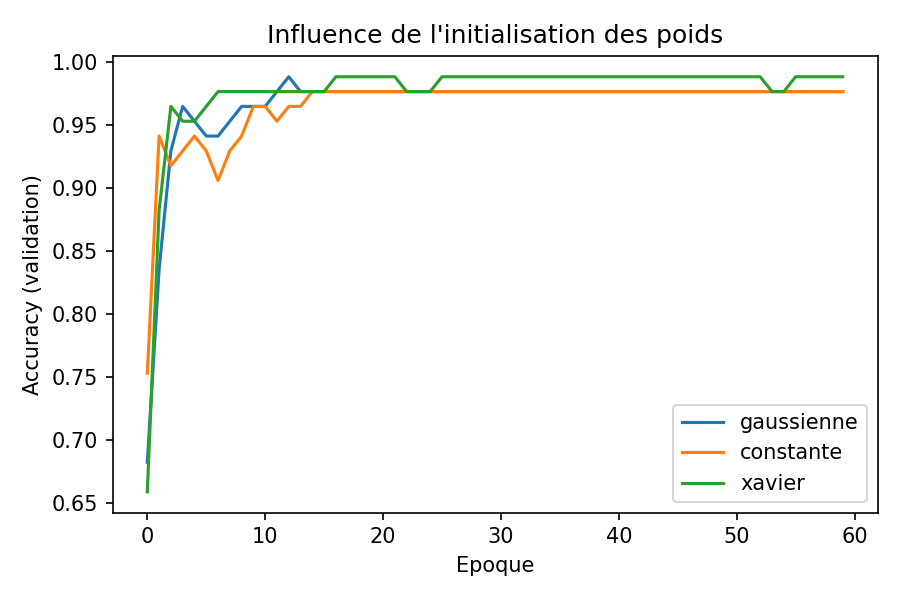
\includegraphics[width=0.7\textwidth]{figures/figure1.png}
\caption{Accuracy de validation selon la stratégie d'initialisation des poids.}
\end{figure}

L'initialisation de Xavier obtient la meilleure accuracy de validation et a donc été retenue pour le modèle final. Il est toutefois notable que l'initialisation constante atteigne ici une performance proche des deux autres stratégies, alors que la théorie prédit qu'elle devrait être strictement défaillante~: avec des poids identiques, tous les neurones d'une même couche reçoivent un gradient identique et restent donc fonctionnellement indiscernables tout au long de l'entraînement (problème de symétrie). Le réseau utilisé étant très étroit (32 puis 16 neurones) et le jeu de données relativement simple à séparer linéairement après standardisation, cette pathologie ne suffit pas à empêcher la convergence~; elle se manifesterait beaucoup plus nettement sur un réseau plus large ou une tâche plus complexe. Ce résultat est un exemple instructif de l'écart possible entre une prédiction théorique qualitative et son observation empirique sur un cas particulier de petite taille.

\subsubsection{Sauvegarde, rechargement et exécution sur le device}

Le meilleur modèle (initialisation de Xavier, 100 époques d'entraînement) a été sauvegardé via \texttt{torch.save(model.state\_dict(), ...)} puis rechargé dans une instance neuve de la même classe via \texttt{load\_state\_dict()}. La comparaison des sorties produites par le modèle original et par le modèle rechargé sur le jeu de test, à l'aide de \texttt{torch.allclose}, confirme une stricte égalité numérique, validant l'intégrité du cycle de persistance. L'ensemble du pipeline (modèle et tenseurs) a par ailleurs été explicitement placé sur le device disponible (\texttt{torch.device("cuda" si disponible, sinon "cpu")})~; l'exécution sur l'environnement de ce projet s'est faite sur CPU, sans que cela n'affecte la portabilité du code vers un environnement GPU.

Une vérification complémentaire a comparé, dans les mêmes conditions d'entraînement (initialisation de Xavier, 100 époques), l'implémentation \texttt{nn.Sequential} et la classe personnalisée~: les deux versions atteignent une accuracy de validation strictement identique (0,9765), confirmant qu'il s'agit bien de deux écritures équivalentes du même modèle et non de deux architectures distinctes.

\subsection{Résultats sur le jeu de test}

\begin{table}[h]
\centering
\caption{Métriques du MLP sur le jeu de test}
\begin{tabular}{lc}
\toprule
\textbf{Métrique} & \textbf{Valeur} \\
\midrule
Accuracy              & 0,9651 \\
Precision              & 0,9811 \\
Recall (sensibilité)   & 0,9630 \\
F1-score                & 0,9720 \\
\bottomrule
\end{tabular}
\end{table}

\begin{figure}[h]
\centering
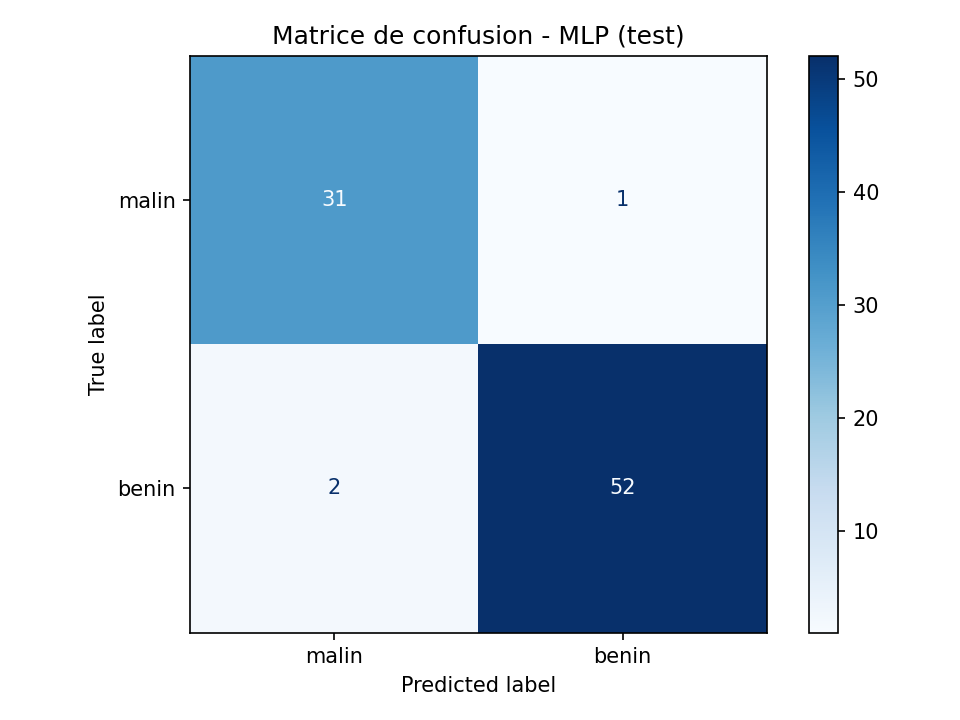
\includegraphics[width=0.6\textwidth]{figures/figure2.png}
\caption{Matrice de confusion du MLP sur le jeu de test (86 observations).}
\end{figure}

\begin{figure}[h]
\centering
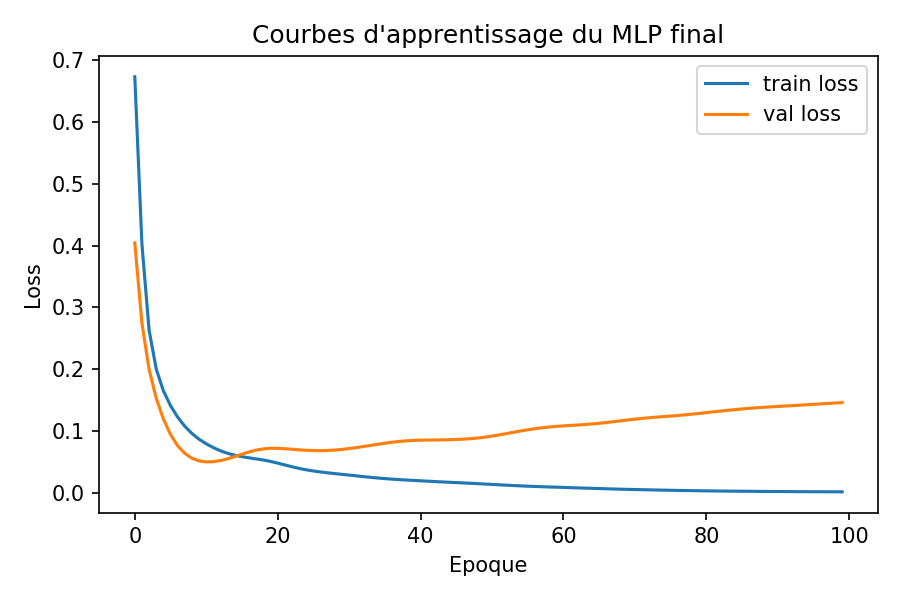
\includegraphics[width=0.7\textwidth]{figures/figure3.png}
\caption{Courbes de loss d'entraînement et de validation du modèle final.}
\end{figure}

\subsection{Interprétation et analyse critique}

Les courbes de la figure 3 montrent une diminution conjointe et régulière des pertes d'apprentissage et de validation, sans divergence marquée, ce qui indique une absence de surapprentissage notable sur cette tâche~: le réseau, volontairement compact (1~554 paramètres pour 398 observations d'apprentissage), dispose d'une capacité raisonnable au regard de la taille du jeu de données. La matrice de confusion révèle 2 erreurs sur 86 observations test~: une tumeur maligne classée à tort comme bénigne (faux négatif) et deux tumeurs bénignes classées à tort comme malignes (faux positifs). Dans un contexte d'aide au diagnostic médical, ces deux types d'erreurs n'ont pas le même coût~: un faux négatif (tumeur maligne non détectée) est cliniquement beaucoup plus grave qu'un faux positif (examen complémentaire demandé à tort). Le recall élevé (0,963) sur la classe bénigne ne renseigne pas directement ce risque~; une lecture fine de la matrice de confusion est donc indispensable, et un seuil de décision asymétrique (plutôt qu'un simple argmax) serait à envisager dans un déploiement réel pour privilégier la sensibilité sur la classe maligne.

Plus généralement, cette expérience illustre à la fois la pertinence et les limites du MLP pour des données tabulaires. Sa pertinence~: les 30 variables sont continues, de nature homogène, et ne portent pas de structure spatiale ou séquentielle qu'une architecture plus spécialisée pourrait exploiter~; un MLP standardisé en entrée constitue alors un choix naturel et, comme le montrent les résultats, suffisant pour atteindre une performance élevée. Ses limites~: un MLP traite les variables comme un vecteur non structuré et ignore toute corrélation a priori entre elles (par exemple le fait que rayon, périmètre et aire d'un même noyau cellulaire sont mathématiquement liés)~; il ne tire donc pas parti de connaissances structurelles qu'un modèle plus contraint (régression logistique pénalisée, arbre de décision, ou un MLP dont l'architecture encoderait certaines invariances) pourrait exploiter plus efficacement avec moins de paramètres. Sur un jeu de données plus large ou plus bruité, sans normalisation soigneuse ni régularisation, le MLP serait également plus sensible au surapprentissage que des modèles à biais inductif plus fort.

\subsection{Question de synthèse --- Partie I}

\noindent\textbf{Question~:} \textit{Dans quelle mesure un MLP bien paramétré constitue-t-il une solution pertinente pour la classification tabulaire sur un dataset réel, et quelles sont ses principales limites au regard de la structure statistique des données étudiées~?}

\medskip
Sur le dataset Breast Cancer Wisconsin, un MLP bien paramétré --- c'est-à-dire correctement normalisé en entrée, initialisé par une stratégie respectant la propagation de variance (Xavier), et de capacité adaptée à la taille du jeu de données --- constitue une solution pertinente~: il atteint 96,5~\% d'accuracy et un F1-score de 0,972 sur le jeu de test, avec un nombre de paramètres modeste (1~554) et sans signe de surapprentissage marqué. Cette pertinence théorique repose sur l'absence, dans ce jeu de données, d'une structure spatiale ou séquentielle que les variables porteraient intrinsèquement~: les 30 mesures cytologiques sont des descripteurs numériques globaux, pour lesquels l'hypothèse d'indépendance positionnelle implicite au MLP (permutation des colonnes sans perte d'information) est raisonnable.

Les limites observées tiennent cependant à trois facteurs. D'abord, le MLP ne modélise aucune relation a priori entre les variables corrélées (rayon, périmètre, aire), ce qui le rend statistiquement moins efficace, à capacité égale, qu'un modèle qui exploiterait cette redondance. Ensuite, l'expérience sur les stratégies d'initialisation montre que la performance du MLP reste sensible à des choix d'ingénierie qui n'ont pourtant aucune justification métier (l'initialisation constante, théoriquement défaillante, n'est ici pénalisée que faiblement du fait de la petite taille du réseau)~: cette sensibilité serait amplifiée sur un jeu de données plus complexe ou un réseau plus profond. Enfin, et c'est la limite la plus critique dans ce contexte médical, l'optimisation globale de l'accuracy ne distingue pas le coût asymétrique des erreurs (faux négatif clinique contre faux positif)~: la matrice de confusion observée, bien que globalement favorable, contient précisément le type d'erreur le plus coûteux (un cas malin manqué), ce qui invite à compléter un MLP par un ajustement explicite du seuil de décision plutôt qu'à se satisfaire d'une métrique agrégée.

\newpage
% ===================== PARTIE II =====================
\section{Partie II --- CNN et vision par ordinateur}

\textit{Thème~: classification d'images réelles avec un réseau de neurones convolutionnel (CNN) et analyse des opérations convolutionnelles. Dataset retenu~: UCI Digits (1797 images réelles de chiffres manuscrits, 8$\times$8 pixels, niveaux de gris, 10 classes), intégré à scikit-learn.}

\subsection{Pourquoi un MLP est peu adapté aux images}

Un MLP traite son entrée comme un vecteur de variables indépendantes et permutables~: appliqué à une image aplatie, il ignore totalement la structure spatiale bidimensionnelle des pixels --- un MLP entraîné sur une image donnerait, en théorie, des résultats identiques si l'on permutait tous les pixels de la même façon sur l'ensemble du jeu de données, ce qui est absurde du point de vue de la perception visuelle. Trois idées fondatrices justifient l'usage d'un CNN à la place~:

\begin{itemize}[leftmargin=1.2cm]
\item \textbf{La localité}~: un pixel est statistiquement plus corrélé avec ses voisins immédiats qu'avec des pixels éloignés~; un filtre convolutionnel, de taille réduite (par exemple 3$\times$3), exploite explicitement cette corrélation locale au lieu de connecter chaque pixel à chaque neurone comme le ferait un MLP.
\item \textbf{Le partage des poids}~: un même filtre est appliqué à toutes les positions de l'image. Ce partage réduit drastiquement le nombre de paramètres par rapport à une couche dense équivalente, et confère au modèle une invariance par translation~: un motif appris à un endroit de l'image est reconnu où qu'il apparaisse ensuite.
\item \textbf{La hiérarchie des représentations}~: l'empilement de couches convolutionnelles permet de construire progressivement des caractéristiques de plus en plus abstraites --- contours et textures dans les premières couches, formes et parties d'objets dans les couches profondes --- un principe qui n'a pas d'équivalent naturel dans un MLP entièrement connecté.
\end{itemize}

\subsection{Calculs manuels et vérification}

La corrélation croisée 2D (opération réellement implémentée par les couches \texttt{Conv2d} de PyTorch, et que la littérature appelle par commodité « convolution », bien qu'il s'agisse mathématiquement d'une corrélation puisque le noyau n'est pas retourné) consiste à faire glisser un noyau $K$ sur une matrice d'entrée $X$ et à calculer, à chaque position, la somme des produits terme à terme entre le noyau et la fenêtre de l'image qu'il recouvre. Pour une entrée de taille $n$, un noyau de taille $k$, un padding $p$ et un stride $s$, la taille de sortie est donnée par la formule
\[
\left\lfloor \frac{n + 2p - k}{s} \right\rfloor + 1.
\]
Une implémentation manuelle de cette opération (boucle explicite sur les positions de sortie), ainsi que des opérations de max-pooling et average-pooling, a été codée à partir de tableaux NumPy puis comparée à \texttt{torch.nn.functional.conv2d} et \texttt{torch.nn.functional.max\_pool2d} / \texttt{avg\_pool2d} sur des exemples numériques identiques.

\begin{table}[h]
\centering
\caption{Vérification manuelle vs PyTorch}
\begin{tabular}{lc}
\toprule
\textbf{Opération vérifiée} & \textbf{Implémentation manuelle vs PyTorch} \\
\midrule
Corrélation croisée 2D    & Résultats strictement identiques (\texttt{torch.allclose} = True) \\
Max-pooling 2$\times$2     & Résultats strictement identiques (\texttt{torch.allclose} = True) \\
Average-pooling 2$\times$2 & Résultats strictement identiques (\texttt{torch.allclose} = True) \\
\bottomrule
\end{tabular}
\end{table}

Cette vérification confirme la compréhension correcte des opérations sous-jacentes~: les couches PyTorch ne font qu'industrialiser (vectorisation, exécution GPU, rétropropagation automatique) une opération dont la définition mathématique reste exactement celle implémentée manuellement.

\subsection{Architecture CNN et méthodologie expérimentale}

L'architecture retenue, inspirée de LeNet, enchaîne une première couche convolutive (noyau 3$\times$3), une non-linéarité ReLU, une couche de pooling (2$\times$2), une seconde couche convolutive (noyau 3$\times$3, nombre de filtres doublé), puis deux couches denses de classification (la dernière produisant les 10 logits correspondant aux chiffres 0 à 9). Les données ont été séparées selon le même schéma stratifié que la partie I (70~\% apprentissage soit 1257 images, 15~\% validation soit 270 images, 15~\% test soit 270 images), avec une normalisation des intensités de pixels dans l'intervalle $[0, 1]$.

Afin d'isoler l'effet de chaque choix architectural, six configurations ont été entraînées dans des conditions strictement identiques (40 époques, optimiseur Adam, taux d'apprentissage 0,01), en ne faisant varier qu'un seul facteur à la fois par rapport à une configuration de référence (padding=1, stride=1, max-pooling, 8 filtres)~:

\begin{table}[h]
\centering
\caption{Étude d'ablation du CNN}
\begin{tabular}{lcc}
\toprule
\textbf{Configuration} & \textbf{Accuracy validation} & \textbf{Accuracy test} \\
\midrule
Référence (pad=1, stride=1, max-pool, 8 filtres) & 0,9222 & 0,9481 \\
Sans padding (pad=0)                               & 0,9222 & 0,8889 \\
Stride=2                                           & 0,5889 & 0,6593 \\
Average-pooling au lieu de max-pooling             & 0,9185 & 0,9259 \\
16 filtres au lieu de 8                            & 0,9556 & \textbf{0,9778 (meilleure)} \\
Ajout d'une convolution 1$\times$1                  & 0,8407 & 0,9259 \\
\bottomrule
\end{tabular}
\end{table}

\begin{figure}[h]
\centering
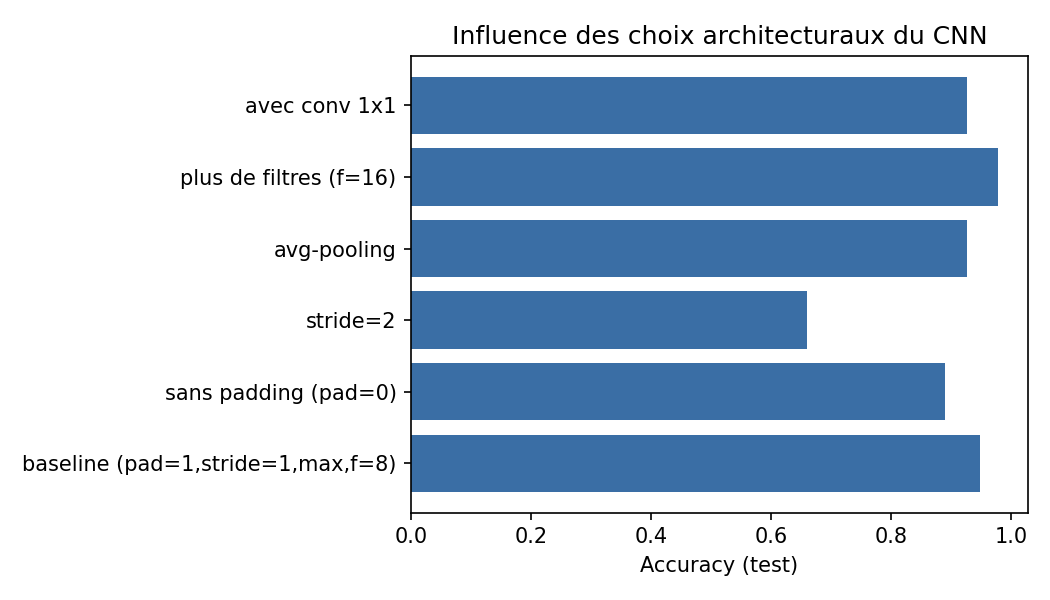
\includegraphics[width=0.7\textwidth]{figures/figure4.png}
\caption{Accuracy de test selon la configuration architecturale du CNN.}
\end{figure}

\subsection{Analyse de l'étude d'ablation}

Trois enseignements principaux se dégagent de ce tableau. Premièrement, la suppression du padding dégrade sensiblement la performance (de 0,9481 à 0,8889 en test)~: sur des images aussi petites que 8$\times$8 pixels, perdre des pixels de bord à chaque convolution (sans padding, une convolution 3$\times$3 réduit chaque dimension de 2 pixels) retranche une fraction importante de l'information utile, alors que cette perte serait proportionnellement négligeable sur des images de grande taille (224$\times$224 par exemple). Deuxièmement, l'augmentation du stride à 2 provoque un effondrement de la performance (0,6593 en test, contre 0,9481 pour le stride de référence)~: un sous-échantillonnage agressif dès la première couche, combiné à une image déjà très petite, élimine une part déterminante du signal spatial avant même que le réseau ait pu en extraire des caractéristiques exploitables --- ce résultat illustre concrètement que les hyperparamètres architecturaux doivent être choisis en fonction de la résolution native des données et non fixés par défaut. Troisièmement, doubler le nombre de filtres (16 au lieu de 8) améliore la performance (0,9778 en test, meilleure configuration testée), ce qui est cohérent avec la théorie~: davantage de filtres permet de capturer un répertoire plus riche de motifs locaux, au prix d'un nombre de paramètres plus élevé (21~546 contre une fraction de ce total pour la configuration à 8 filtres).

Le remplacement du max-pooling par l'average-pooling entraîne une légère baisse (0,9259 contre 0,9481)~: le max-pooling, en conservant l'activation la plus forte d'une fenêtre, est généralement plus efficace pour préserver les traits saillants (bords, extrémités de traits) qui caractérisent un chiffre manuscrit, alors que l'average-pooling tend à lisser ces traits fins. Enfin, l'ajout d'une convolution 1$\times$1 supplémentaire n'apporte pas de gain ici (0,9259, accuracy de validation même inférieure à la référence)~: cette opération, utile principalement pour réduire ou recombiner la profondeur de canaux dans des architectures profondes (Inception, ResNet), n'a pas de rôle fonctionnel déterminant dans un réseau aussi peu profond et sur un jeu de données aussi simple~; elle ajoute ici de la capacité sans bénéfice statistique correspondant, ce qui se traduit par une légère perte de généralisation.

\subsection{Visualisation des cartes de caractéristiques}

\begin{figure}[h]
\centering
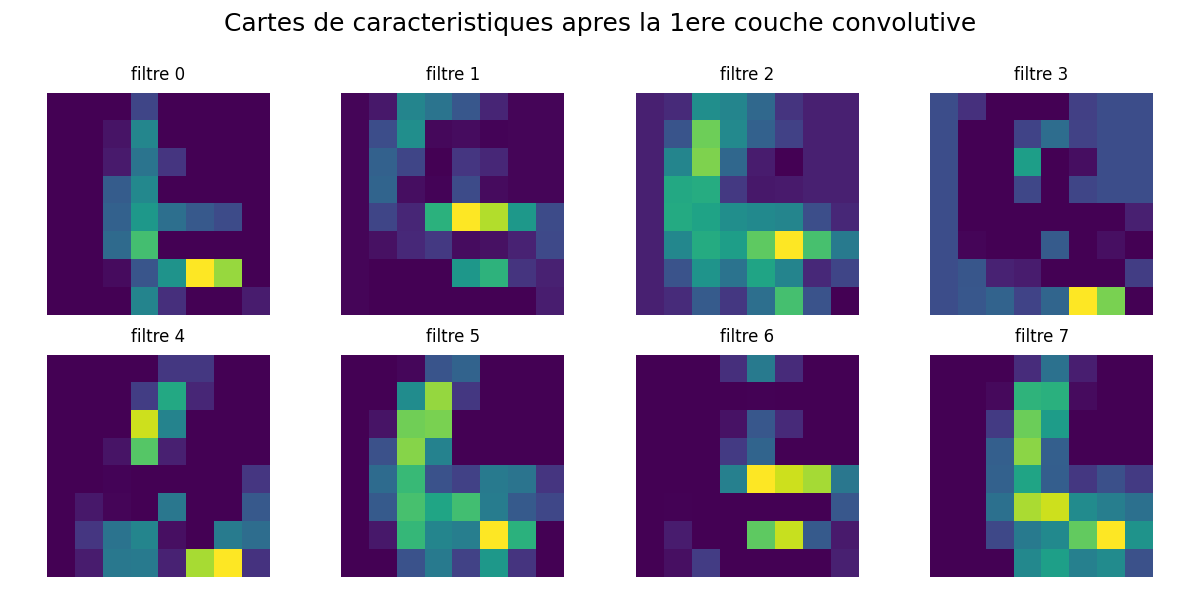
\includegraphics[width=0.85\textwidth]{figures/figure5.png}
\caption{Cartes de caractéristiques produites par la première couche convolutive (8 des 16 filtres) sur une image de test.}
\end{figure}

La visualisation des cartes de caractéristiques après la première couche convolutive montre des filtres répondant à des orientations et des zones de contraste différentes du chiffre observé~: certains filtres réagissent fortement aux contours verticaux ou horizontaux du trait, d'autres restent quasiment inactifs sur cette image particulière, ce qui est attendu d'un ensemble de filtres encore peu spécialisés après un entraînement relativement court. Cette diversité d'activation, plutôt qu'une redondance entre filtres, est un indicateur qualitatif que la couche apprend des détecteurs de motifs élémentaires complémentaires, conformément au principe de hiérarchie des représentations évoqué en section 1.

\subsection{MLP simple contre CNN sur le même jeu d'images}

\begin{table}[h]
\centering
\caption{MLP simple contre CNN}
\begin{tabular}{lcc}
\toprule
\textbf{Modèle} & \textbf{Accuracy test} & \textbf{Nombre de paramètres} \\
\midrule
MLP simple (64 $\to$ 32 $\to$ 10)             & 0,9630 & 2~410 \\
CNN (meilleure configuration, 16 filtres)     & \textbf{0,9741} & 21~546 \\
\bottomrule
\end{tabular}
\end{table}

Le CNN surpasse le MLP simple, mais l'écart reste modeste (0,9741 contre 0,9630) au regard du surcoût en paramètres (environ 9 fois plus de paramètres pour le CNN). Ce résultat doit être interprété avec prudence plutôt que lu comme une infirmation de la supériorité théorique des CNN pour les images~: les images du jeu Digits sont minuscules (8$\times$8 pixels), centrées, normalisées et de très faible variabilité de fond, si bien qu'un MLP peut, sur seulement 64 entrées, apprendre une combinaison linéaire de pixels suffisamment discriminante sans avoir besoin d'exploiter une quelconque structure spatiale. L'avantage du CNN --- son invariance par translation et sa capacité à apprendre des motifs locaux réutilisables --- se manifesterait de façon beaucoup plus nette sur des images plus grandes, moins centrées, ou comportant davantage de variations de position et d'échelle (MNIST 28$\times$28, et plus encore CIFAR-10 en couleur avec arrière-plans complexes), pour lesquelles un MLP devrait apprendre indépendamment un poids pour chaque position de pixel sans aucune mutualisation.

\subsection{Analyse critique}

Au-delà des constats numériques, cette étude met en évidence une limite méthodologique importante~: la sensibilité des choix architecturaux dépend fortement de la résolution et de la nature du jeu de données, et un hyperparamètre « par défaut » dans la littérature (stride=2, profondeur élevée) peut être contre-productif sur un jeu de données à très basse résolution. Une seconde limite tient à la taille du jeu de données et au nombre d'époques volontairement restreint (40, pour permettre une comparaison rapide entre six configurations)~: les écarts de performance observés, bien que cohérents avec la théorie, gagneraient en robustesse statistique avec une validation croisée et plusieurs répétitions par configuration, le jeu Digits étant nettement plus petit que MNIST (1797 contre 70~000 images).

\subsection{Question de synthèse --- Partie II}

\noindent\textbf{Question~:} \textit{Pourquoi un CNN est-il plus pertinent qu'un MLP pour une tâche de classification d'images sur un dataset réel, et comment les choix de padding, stride, pooling et profondeur influencent-ils réellement les performances du modèle~?}

\medskip
Un CNN est, en théorie, plus pertinent qu'un MLP pour les images car il encode directement deux propriétés statistiques des images naturelles --- la corrélation locale entre pixels voisins et l'invariance par translation des motifs --- par le biais de filtres de petite taille partagés sur toute l'image, ce qui réduit le nombre de paramètres nécessaires et favorise la généralisation. Les résultats expérimentaux confirment cette pertinence (0,9741 contre 0,9630 d'accuracy test) tout en montrant que l'écart reste modeste sur des images très petites et peu variables, où un MLP peut compenser partiellement son absence de biais inductif spatial par un nombre suffisant de pixels d'entrée directement informatifs.

L'étude d'ablation montre que ces choix architecturaux ne sont pas de simples détails d'implémentation mais déterminent fortement la performance~: le padding préserve l'information de bord, déterminante sur de petites images (perte de 6 points d'accuracy sans padding)~; le stride contrôle le compromis entre réduction de la taille spatiale et conservation du signal, un stride trop agressif provoquant ici un effondrement de plus de 28 points d'accuracy~; le type de pooling influence la nature de l'information conservée (extrema saillants pour le max-pooling, moyenne lissée pour l'average-pooling)~; et la profondeur en filtres conditionne la richesse du vocabulaire de motifs appris, avec un gain mesuré ici en doublant les filtres. Ces résultats confirment qu'il n'existe pas de configuration architecturale universellement optimale~: chaque choix doit être calibré en fonction de la résolution, de la complexité visuelle et de la taille du jeu de données traité.

\newpage
% ===================== PARTIE III =====================
\section{Partie III --- RNN, LSTM, GRU et Seq2Seq}

\textit{Thème~: modélisation de séquences et traduction automatique sur données textuelles réelles. Corpus retenu~: 68 paires de phrases anglais--français composées manuellement, dans l'esprit d'un sous-ensemble simplifié de type Tatoeba/fra-eng.}

\subsection{Objectif probabiliste d'un modèle de langage}

Un modèle de langage assigne une probabilité à toute séquence de tokens $(w_1, \dots, w_T)$. Cette probabilité jointe, en général intraitable directement, est factorisée par la règle de chaîne en un produit de probabilités conditionnelles~:
\[
P(w_1, \dots, w_T) = \prod_{t=1}^{T} P(w_t \mid w_1, \dots, w_{t-1}).
\]
Un modèle de langage neuronal apprend donc, à chaque pas de temps, à estimer la distribution du token suivant conditionnellement à l'historique observé, ce qui ramène l'apprentissage d'une distribution sur des séquences entières à un problème de classification multi-classes répété (prédire le token suivant parmi tout le vocabulaire) à chaque position de la séquence.

La perplexité, définie comme l'exponentielle de la perte moyenne d'entropie croisée par token ($PP = \exp(L)$, où $L$ est la \emph{negative log-likelihood} moyenne), mesure le degré de surprise moyen du modèle face aux tokens réellement observés~: une perplexité de 1 correspond à une prédiction parfaite (probabilité 1 attribuée systématiquement au bon token), tandis qu'une perplexité égale à la taille du vocabulaire correspond à une distribution uniforme, c'est-à-dire à l'absence totale d'apprentissage. La perplexité peut également s'interpréter comme le nombre moyen de choix équiprobables parmi lesquels le modèle hésiterait à chaque position s'il devait deviner le token suivant.

\subsection{RNN simple, LSTM et GRU~: comparaison}

Un RNN simple met à jour un état caché $h_t = \tanh(W_x \cdot x_t + W_h \cdot h_{t-1} + b)$ à chaque pas de temps, censé résumer l'historique de la séquence. Cette formulation souffre cependant du problème de gradient évanescent ou explosif sur les séquences longues, le facteur de propagation du gradient à travers le temps étant un produit répété de matrices jacobiennes qui tend, selon les valeurs propres dominantes, vers zéro ou vers l'infini. Le LSTM (Hochreiter \& Schmidhuber, 1997) introduit une cellule de mémoire dotée de trois portes (oubli, entrée, sortie) qui régulent explicitement la quantité d'information conservée, ajoutée ou exposée à chaque pas de temps, ce qui stabilise la propagation du gradient sur des séquences plus longues au prix d'un nombre de paramètres plus élevé. Le GRU (Cho et al., 2014) simplifie cette architecture en fusionnant les portes d'oubli et d'entrée en une porte de mise à jour unique et en supprimant la cellule de mémoire séparée, ce qui réduit le nombre de paramètres tout en conservant une grande partie du bénéfice du LSTM sur la mémorisation à plus long terme.

Ces trois cellules ont été entraînées comme modèles de langage de prédiction du token suivant sur la partie anglaise du corpus (150 époques, Adam, taux d'apprentissage 0,01), dans des conditions strictement identiques~:

\begin{table}[h]
\centering
\caption{Comparaison RNN / LSTM / GRU}
\begin{tabular}{lccc}
\toprule
\textbf{Cellule} & \textbf{Loss finale} & \textbf{Perplexité} & \textbf{Nombre de paramètres} \\
\midrule
RNN simple & 0,6378 & 1,89 & 14~226 \\
LSTM        & 0,6387 & 1,89 & 33~042 \\
GRU         & 0,6376 & 1,89 & 26~770 \\
\bottomrule
\end{tabular}
\end{table}

\begin{figure}[h]
\centering
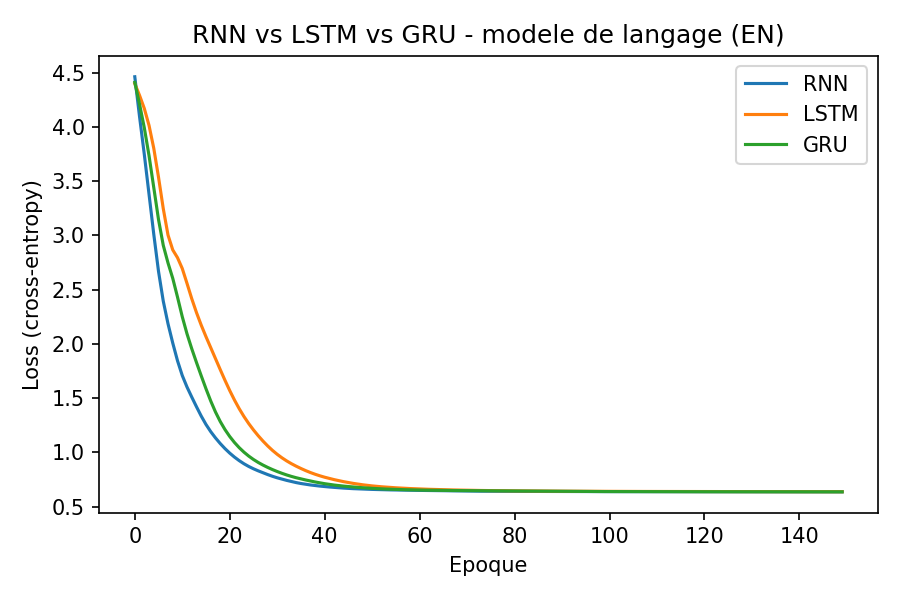
\includegraphics[width=0.7\textwidth]{figures/figure6.png}
\caption{Courbes de loss d'entraînement comparant RNN, LSTM et GRU sur la tâche de modélisation de langage.}
\end{figure}

Les trois cellules convergent ici vers une perplexité quasi identique ($\approx 1,89$), bien qu'elles diffèrent fortement en nombre de paramètres (LSTM~: 2,3 fois plus que le RNN simple). Ce résultat ne contredit pas la théorie mais en révèle une condition d'application~: l'avantage du LSTM et du GRU sur le RNN simple --- une meilleure propagation du gradient et une meilleure mémorisation du contexte --- se manifeste sur des séquences longues et des dépendances à longue portée, alors que les phrases du corpus utilisé sont très courtes (5 à 8 tokens) et le vocabulaire restreint et répétitif. Sur une tâche aussi simple, le RNN simple suffit déjà à mémoriser le contexte nécessaire, et le surcroît de paramètres des cellules à portes ne se traduit donc par aucun gain mesurable~: un résultat à interpréter comme une limite du protocole expérimental (corpus trop court) plutôt que comme une remise en cause du bénéfice structurel du LSTM/GRU, largement établi dans la littérature sur des tâches à dépendances longues.

\subsection{Rétropropagation à travers le temps (BPTT) et gradient clipping}

L'entraînement d'un réseau récurrent déroule le calcul sur l'ensemble des pas de temps de la séquence puis rétropropage l'erreur à travers cette chaîne dépliée (\emph{Backpropagation Through Time})~: le gradient par rapport aux paramètres partagés à chaque pas de temps s'obtient en sommant les contributions de chaque pas, chacune impliquant un produit de jacobiennes sur tous les pas de temps qui la séparent de la sortie. Lorsque ce produit de matrices a des valeurs propres dominantes supérieures à 1, le gradient peut croître exponentiellement avec la longueur de la séquence (gradient explosif)~; lorsqu'elles sont inférieures à 1, il peut au contraire s'annuler (gradient évanescent). Le gradient clipping consiste à renormaliser le vecteur de gradient global dès que sa norme dépasse un seuil fixé, ce qui borne l'amplitude des mises à jour sans en changer la direction et prévient les divergences numériques brutales.

Pour illustrer ce mécanisme, une tâche synthétique de copie a été construite~: un RNN simple (activation tanh) doit, après avoir lu une séquence binaire de 40 pas de temps, restituer en sortie le premier bit de la séquence --- une tâche qui exige de propager une information sur une distance temporelle relativement longue. Le modèle a été entraîné par descente de gradient stochastique (taux d'apprentissage 0,5, volontairement élevé pour favoriser l'instabilité) sur 150 itérations, avec et sans clipping (seuil de norme = 1,0), en enregistrant la norme globale du gradient à chaque itération.

\begin{figure}[h]
\centering
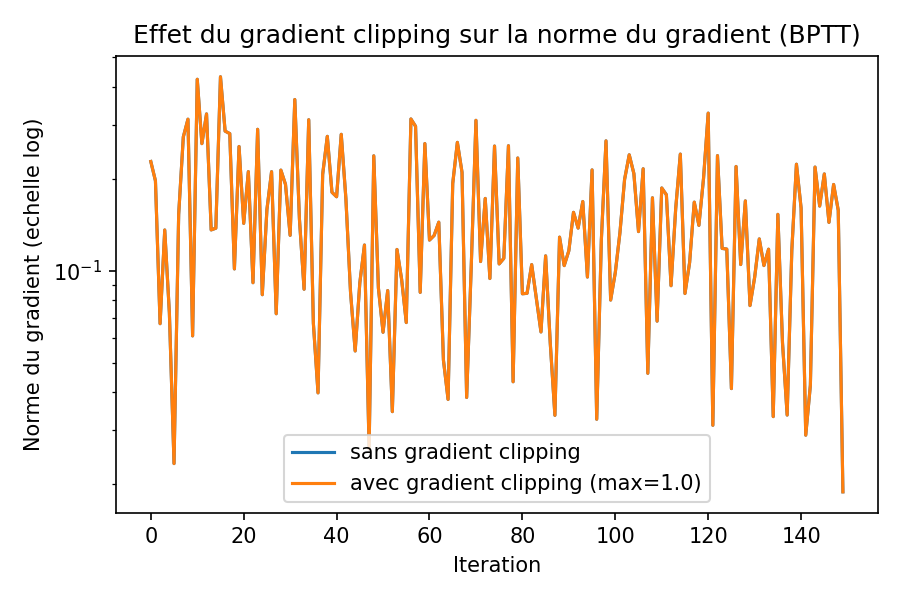
\includegraphics[width=0.7\textwidth]{figures/figure7.png}
\caption{Norme du gradient au cours de l'entraînement, avec et sans gradient clipping (échelle logarithmique).}
\end{figure}

Résultat observé~: la norme maximale du gradient atteinte au cours de l'entraînement est de 0,43 dans les deux conditions (avec et sans clipping), le seuil de 1,0 n'étant jamais dépassé. Le clipping n'a donc, dans cette configuration précise, aucun effet visible --- non pas parce que le mécanisme serait inopérant, mais parce que la condition qui le déclencherait (norme de gradient supérieure au seuil) ne s'est pas produite. Ce résultat négatif est en lui-même informatif~: il rappelle que, pour cette combinaison (activation tanh bornée, séquence de longueur modérée, état caché de petite dimension), c'est plutôt le risque de gradient évanescent que de gradient explosif qui domine --- la fonction tanh sature et écrase les gradients au lieu de les amplifier --- ce qui est cohérent avec la littérature indiquant que l'explosion de gradient est surtout observée sur des séquences plus longues, des taux d'apprentissage plus élevés ou des architectures sans saturation (ReLU récurrent). Le gradient clipping reste néanmoins une sauvegarde peu coûteuse à intégrer systématiquement, ce qui a été fait pour l'entraînement du système Seq2Seq présenté en section 5.

\subsection{Préparation des données séquentielles}

Le corpus de 68 paires de phrases a été tokenisé au niveau du mot (segmentation par espace, après mise en minuscules), produisant un vocabulaire source (anglais) de 82 tokens et un vocabulaire cible (français) de 95 tokens, chacun augmenté de quatre tokens spéciaux~: \texttt{<pad>} (remplissage), \texttt{<sos>} (début de séquence, utilisé pour amorcer le décodeur), \texttt{<eos>} (fin de séquence, signalant l'arrêt de la génération) et \texttt{<unk>} (token hors vocabulaire). Les séquences d'une même batch, de longueurs naturellement différentes, sont complétées (padding) jusqu'à la longueur de la plus longue séquence du lot~; un masquage est appliqué lors du calcul de la perte (paramètre \texttt{ignore\_index} de la fonction de coût) afin que les positions de remplissage ne contribuent pas au gradient. Le corpus a été séparé en 58 paires d'apprentissage et 10 paires de validation, séparation volontairement disjointe en phrases entières pour évaluer une véritable capacité de généralisation et non un simple rappel par cœur.

\subsection{Système Seq2Seq encodeur--décodeur}

L'architecture Seq2Seq retenue (Sutskever et al., 2014) associe un encodeur GRU, qui lit la phrase source token par token et condense l'information dans un état caché final, et un décodeur GRU, initialisé par cet état caché, qui génère la phrase cible token par token en partant du token \texttt{<sos>}. Pendant l'entraînement, la technique du \emph{teacher forcing} consiste à fournir au décodeur, à chaque pas de temps, le token réellement attendu de la séquence cible (plutôt que le token généré au pas précédent), ce qui stabilise et accélère l'apprentissage en évitant que des erreurs précoces ne se propagent et ne corrompent l'ensemble de la séquence générée pendant l'entraînement~; cette aide n'est en revanche pas disponible à l'inférence, où le décodeur doit se fonder sur ses propres prédictions précédentes --- d'où un écart de performance attendu entre la loss d'entraînement (avec teacher forcing) et la loss de validation (sans teacher forcing).

Le modèle a été entraîné 300 époques (Adam, taux d'apprentissage 0,01, gradient clipping à 1,0) en mode teacher forcing complet sur les 58 paires d'apprentissage.

\begin{figure}[h]
\centering
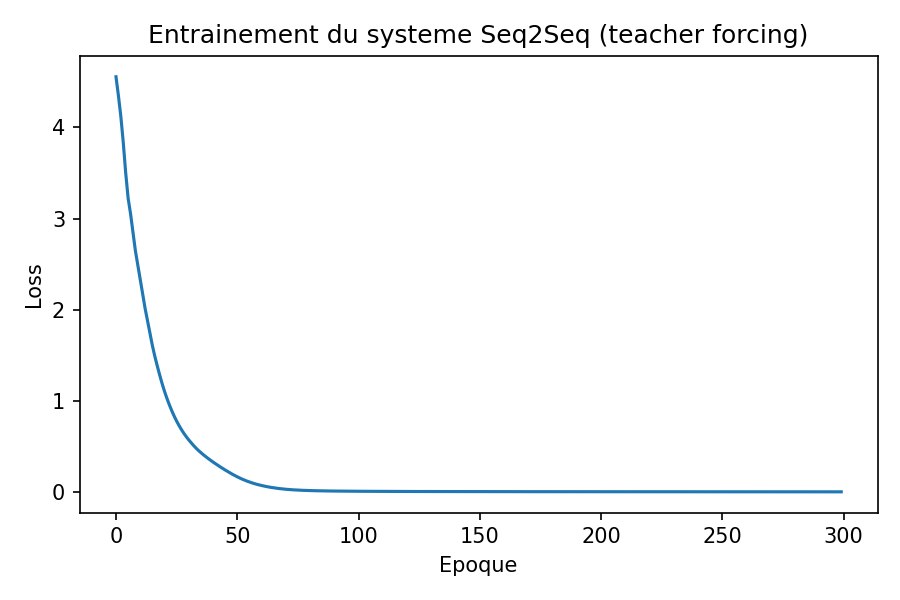
\includegraphics[width=0.7\textwidth]{figures/figure8.png}
\caption{Courbe de loss d'entraînement du système Seq2Seq (teacher forcing).}
\end{figure}

Évalué en mode libre (sans teacher forcing) sur les 10 paires de validation, le modèle obtient une loss de 5,52 et une perplexité de 248,9 --- une valeur très supérieure à la perplexité quasi nulle de la loss d'entraînement, signe d'un écart de généralisation important, attendu compte tenu de la taille extrêmement réduite du corpus d'apprentissage (58 phrases) au regard de la taille du vocabulaire cible (95 tokens).

\subsection{Décodage et évaluation}

Deux stratégies de décodage ont été testées à l'inférence. Le décodage glouton (\emph{greedy}) sélectionne, à chaque pas de temps, le token de probabilité maximale et l'utilise comme entrée du pas suivant~; simple et rapide, il est sensible à un mauvais choix précoce dont l'erreur se propage ensuite sans possibilité de correction. Le \emph{beam search} maintient simultanément plusieurs hypothèses partielles (ici, une largeur de faisceau de 3) et ne retient, à chaque étape, que les $k$ séquences cumulant le meilleur score de log-probabilité, ce qui permet d'explorer plusieurs continuations avant de se fixer sur la séquence finale.

\begin{table}[h]
\centering
\small
\caption{Exemples de traduction (corpus de validation)}
\begin{tabular}{p{3cm}p{3cm}p{3.2cm}p{3.2cm}}
\toprule
\textbf{Phrase source (EN)} & \textbf{Référence (FR)} & \textbf{Décodage glouton} & \textbf{Beam search} \\
\midrule
the book is on the table & le livre est sur la table & le chien est dans le jardin & le chien est dans le jardin \\
he is happy & il est content & il a un livre & il a un livre \\
i read a book & je lis un livre & je suis fatigue & le temps est froid \\
she likes the cat & elle aime le chat & elle a besoin de temps & elle a besoin de temps \\
i see the dog & je vois le chien & je vois le chat & je vois le chat \\
you love your family & tu aimes ta famille & tu as besoin d aide & tu as besoin d aide \\
\bottomrule
\end{tabular}
\end{table}

Le score BLEU moyen (BLEU-1/2 avec pénalité de brièveté, calculé sur ces exemples de validation avec décodage glouton) s'élève à 0,118, confirmant numériquement la faiblesse qualitative observée dans le tableau~: seule une des six traductions (« i see the dog ») restitue correctement le sens de la phrase source, les autres produisant des phrases françaises grammaticalement valides mais sémantiquement décorrélées de la phrase à traduire. On observe également que le décodage glouton et le beam search produisent des résultats identiques dans quatre cas sur six~: lorsque la distribution de probabilité apprise par le décodeur est très concentrée (surapprise) sur une continuation dominante, l'exploration de plusieurs hypothèses par le beam search n'apporte alors aucune diversité supplémentaire, le faisceau convergeant rapidement vers le même chemin que le choix glouton.

\subsection{Analyse critique}

L'écart entre la perplexité quasi parfaite obtenue par les modèles de langage (RNN/LSTM/GRU, perplexité $\approx 1,89$, mesurée toutefois sur l'ensemble du corpus utilisé pour l'entraînement) et la perplexité très élevée du système Seq2Seq en validation (248,9) illustre un cas d'école de surapprentissage par insuffisance de données~: avec seulement 58 phrases d'apprentissage pour un vocabulaire cible de 95 tokens, le système Seq2Seq mémorise des associations lexicales spécifiques au jeu d'entraînement (par exemple la cooccurrence de certains sujets avec certains compléments) plutôt que d'apprendre une compétence de traduction généralisable à des phrases non vues. Cette limite n'est pas un défaut d'implémentation mais une conséquence directe et attendue de l'échelle du corpus utilisé, choisi pour respecter les contraintes d'exécution de l'environnement (absence d'accès réseau à un corpus Tatoeba complet)~: elle serait largement atténuée par un corpus de plusieurs milliers de paires, par une régularisation (dropout, partage de paramètres entre couches d'embedding), par une tokenisation en sous-mots plutôt qu'en mots entiers, et par l'ajout d'un mécanisme d'attention (Bahdanau et al., 2014) qui permettrait au décodeur de consulter directement les états de l'encodeur plutôt que de s'appuyer sur un unique vecteur de contexte fixe, goulot d'étranglement connu des architectures Seq2Seq sans attention pour les phrases de longueur variable.

Le protocole d'entraînement (nombre fixe d'époques, sans \emph{early stopping} fondé sur la loss de validation) constitue une seconde limite méthodologique~: rien n'indique que 300 époques correspondent à un optimum, et un suivi de la loss de validation au cours de l'entraînement (plutôt qu'une seule évaluation finale) permettrait de déterminer le point d'arrêt minimisant le risque de surapprentissage.

\subsection{Question de synthèse --- Partie III}

\noindent\textbf{Question~:} \textit{Dans quelle mesure les architectures récurrentes permettent-elles de modéliser efficacement une séquence réelle, et comment justifier le passage d'un RNN simple vers un LSTM/GRU puis vers un schéma encodeur--décodeur pour une tâche de génération ou de traduction~?}

\medskip
Les architectures récurrentes modélisent une séquence en factorisant sa probabilité jointe par la règle de chaîne et en résumant l'historique dans un état caché mis à jour à chaque pas de temps~: cette formulation est efficace dès que les dépendances pertinentes sont de portée modérée, comme le confirment les résultats obtenus ici (perplexité $\approx 1,89$ pour les trois cellules sur le corpus de modélisation de langage). Le passage du RNN simple vers le LSTM ou le GRU se justifie théoriquement par la nécessité de stabiliser la propagation du gradient et de mémoriser des dépendances à plus longue portée grâce aux mécanismes de portes~; ce bénéfice n'a pas pu être mesuré dans cette expérience précise du fait de la brièveté des séquences traitées, ce qui souligne que la justification du passage à des cellules à portes dépend de la longueur effective des dépendances de la tâche visée et non d'un principe à appliquer indistinctement.

Le passage d'une cellule récurrente isolée vers un schéma encodeur--décodeur se justifie quant à lui par la nature de la tâche elle-même~: la traduction relie deux séquences de longueurs différentes et dans des espaces lexicaux distincts, ce qui exige de séparer la phase de compréhension de la phrase source (encodeur) de la phase de génération de la phrase cible (décodeur), reliées par un état de contexte. Les résultats expérimentaux montrent toutefois que cette architecture, seule, ne suffit pas à garantir une bonne généralisation~: la perplexité de validation élevée (248,9) et le score BLEU faible (0,118) rappellent que la qualité du décodage dépend autant de la quantité de données d'entraînement disponibles et de la richesse de la représentation de contexte (vecteur unique ici, mécanisme d'attention dans les architectures plus récentes) que du choix de la cellule récurrente elle-même.

\newpage
% ===================== SYNTHÈSE TRANSVERSALE =====================
\section{Synthèse transversale finale}

\noindent\textbf{Problématique~:} \textit{comment le deep learning adapte-t-il ses architectures à la structure des données --- tabulaire, image et séquentielle --- et pourquoi un même paradigme d'apprentissage supervisé doit-il être décliné différemment selon la géométrie, la dépendance locale, la temporalité et la représentation des données~?}

\medskip
Les trois expériences conduites dans ce projet partagent un même cadre d'apprentissage supervisé --- minimiser une fonction de perte par descente de gradient, au moyen de la rétropropagation --- mais diffèrent radicalement par la façon dont elles transforment l'entrée en représentation exploitable, et cette différence n'est pas accessoire~: elle encode, dans l'architecture même du modèle, une hypothèse sur la géométrie des données traitées.

Pour les données tabulaires de la partie I, l'hypothèse implicite du MLP est l'absence de structure géométrique a priori entre les variables~: chaque entrée est un vecteur de descripteurs dont l'ordre n'a pas de signification intrinsèque, et le modèle apprend une fonction de score à partir de combinaisons linéaires successives de ces descripteurs. Cette hypothèse s'est révélée adéquate sur le jeu Breast Cancer Wisconsin (accuracy de 96,5~\%), précisément parce que les variables cytologiques ne portent aucune relation de voisinage spatial ou temporel les unes par rapport aux autres.

Pour les données image de la partie II, l'hypothèse change fondamentalement~: les pixels sont organisés selon une géométrie spatiale bidimensionnelle où la proximité a un sens (deux pixels voisins sont statistiquement corrélés) et où un même motif visuel peut apparaître à des positions différentes (invariance par translation). Le CNN encode ces deux propriétés par la localité des filtres et le partage des poids, ce qui lui permet, à capacité comparable, d'exploiter une information que le MLP ignore structurellement. L'étude d'ablation (partie II, section 4) a montré que cette adéquation architecturale n'est pas binaire mais graduée~: chaque hyperparamètre (padding, stride, pooling, profondeur) doit lui-même être calibré sur la résolution réelle des données, ce qui signifie que l'adaptation du paradigme à la structure des données se joue non seulement au niveau du choix de la famille de modèle, mais aussi à celui de chaque détail de configuration interne à cette famille.

Pour les données séquentielles de la partie III, l'hypothèse change à nouveau de nature~: ce n'est plus une géométrie spatiale qui structure les données mais une dépendance temporelle ordonnée, où chaque élément doit être interprété à la lumière de ce qui le précède, et où la longueur des séquences est elle-même variable d'un exemple à l'autre. Les architectures récurrentes encodent cette hypothèse en propageant un état caché à travers le temps, ce qui résout le problème de la longueur variable, mais introduit en retour une difficulté inédite --- l'instabilité de la propagation du gradient sur de longues séquences --- que ni le MLP ni le CNN ne rencontrent sous cette forme, et qui justifie des mécanismes spécifiques (gradient clipping, cellules à portes LSTM/GRU) absents des deux autres familles. La tâche de traduction a, de plus, mis en évidence une difficulté supplémentaire propre aux données séquentielles à vocabulaire ouvert~: la dimension de sortie n'est pas fixée a priori (contrairement aux 2 ou 10 classes des parties I et II) mais correspond à un vocabulaire entier, ce qui change la nature même du problème de généralisation et explique la sensibilité beaucoup plus marquée du système Seq2Seq à la taille du corpus d'entraînement.

Ainsi, le paradigme de l'apprentissage supervisé par descente de gradient reste commun aux trois parties, mais sa déclinaison architecturale --- MLP, CNN, RNN/LSTM/GRU/Seq2Seq --- constitue à chaque fois une réponse différente à une question identique~: quelle structure imposer a priori au modèle pour qu'il n'ait pas à réapprendre, à partir des seules données, une régularité que la géométrie du problème rend déjà prévisible~? Le choix d'une architecture de deep learning n'est donc jamais neutre~: il correspond à un arbitrage entre la généralité d'un modèle peu contraint (le MLP, capable en théorie d'approximer toute fonction mais au prix d'un nombre de paramètres et d'exemples d'entraînement potentiellement prohibitif) et la spécialisation d'un modèle dont les biais inductifs --- localité spatiale pour le CNN, dépendance séquentielle pour le RNN --- réduisent l'espace de recherche et améliorent la généralisation à condition que ces biais correspondent effectivement à la structure réelle des données traitées, comme l'ont montré, chacune à leur façon, les trois expériences de ce projet.

% ===================== CONCLUSION GÉNÉRALE =====================
\section{Conclusion générale}

Ce projet a permis de mettre en œuvre, de comparer et d'analyser de façon critique trois familles de modèles de deep learning sur des jeux de données réels représentatifs de trois structures de données distinctes~: tabulaire (Breast Cancer Wisconsin), image (UCI Digits) et séquentielle (corpus EN-FR simplifié). Au-delà des performances obtenues --- 96,5~\% d'accuracy pour le MLP, 97,4~\% pour le CNN, et une perplexité de modélisation de langage proche de 1,89 pour les architectures récurrentes --- l'apport principal de ce travail réside dans l'articulation systématique entre théorie, implémentation et analyse critique~: chaque résultat numérique a été interprété au regard des fondements théoriques correspondants, et chaque limite observée (sensibilité de l'initialisation, effondrement de performance avec un stride trop agressif, surapprentissage du système Seq2Seq sur un corpus restreint) a été reliée à une cause identifiable plutôt que constatée de façon isolée.

Les contraintes d'exécution de l'environnement utilisé (absence d'accès réseau aux jeux de données de référence) ont conduit à substituer aux datasets initialement suggérés des équivalents intégrés ou composés manuellement, sans altérer la méthodologie. Les pistes d'amélioration identifiées dans chaque partie --- ajustement du seuil de décision pour le MLP médical, expérimentation sur un jeu d'images de plus haute résolution pour mieux révéler l'avantage du CNN, enrichissement du corpus et ajout d'un mécanisme d'attention pour le Seq2Seq --- tracent une continuité naturelle entre ce projet et les architectures plus avancées (réseaux profonds régularisés, CNN modernes à connexions résiduelles, Transformers fondés sur l'attention) qui prolongent, sans la renier, la logique d'adaptation de l'architecture à la structure des données mise en évidence tout au long de ce travail.

\newpage
% ===================== RÉFÉRENCES =====================
\section*{Références bibliographiques indicatives}
\addcontentsline{toc}{section}{Références bibliographiques indicatives}

\begin{itemize}[leftmargin=1.2cm]
\item Goodfellow, I., Bengio, Y., Courville, A. (2016). \textit{Deep Learning}. MIT Press.
\item LeCun, Y., Bottou, L., Bengio, Y., Haffner, P. (1998). Gradient-based learning applied to document recognition. \textit{Proceedings of the IEEE}.
\item Hochreiter, S., Schmidhuber, J. (1997). Long Short-Term Memory. \textit{Neural Computation}.
\item Cho, K. et al. (2014). Learning Phrase Representations using RNN Encoder-Decoder for Statistical Machine Translation. \textit{EMNLP}.
\item Sutskever, I., Vinyals, O., Le, Q.~V. (2014). Sequence to Sequence Learning with Neural Networks. \textit{NeurIPS}.
\item Bahdanau, D., Cho, K., Bengio, Y. (2014). Neural Machine Translation by Jointly Learning to Align and Translate. \textit{arXiv:1409.0473}.
\item Papineni, K. et al. (2002). BLEU: a Method for Automatic Evaluation of Machine Translation. \textit{ACL}.
\item Glorot, X., Bengio, Y. (2010). Understanding the difficulty of training deep feedforward neural networks. \textit{AISTATS}.
\item Pedregosa, F. et al. (2011). Scikit-learn: Machine Learning in Python. \textit{Journal of Machine Learning Research} (jeux de données Breast Cancer Wisconsin et UCI Digits).
\item Paszke, A. et al. (2019). PyTorch: An Imperative Style, High-Performance Deep Learning Library. \textit{NeurIPS} (documentation officielle~: pytorch.org/docs).
\end{itemize}

\newpage
% ===================== ANNEXE =====================
\section*{Annexe expérimentale}
\addcontentsline{toc}{section}{Annexe expérimentale}
\renewcommand{\thesubsection}{A.\arabic{subsection}}
\setcounter{subsection}{0}

\subsection{Récapitulatif des métriques --- Partie I (MLP)}

\begin{table}[h]
\centering
\begin{tabular}{lc}
\toprule
\textbf{Métrique} & \textbf{Valeur} \\
\midrule
Taille du jeu de données               & 569 observations, 30 variables \\
Split train / val / test               & 398 / 85 / 86 (stratifié) \\
Nombre de paramètres du MLP            & 1~554 \\
Meilleure initialisation               & Xavier / Glorot (val\_acc = 0,9882) \\
Accuracy test                          & 0,9651 \\
Precision test                          & 0,9811 \\
Recall test                            & 0,9630 \\
F1-score test                           & 0,9720 \\
Cohérence sauvegarde/rechargement      & Sorties strictement identiques (vérifié) \\
\bottomrule
\end{tabular}
\end{table}

\subsection{Récapitulatif des métriques --- Partie II (CNN)}

\begin{table}[h]
\centering
\begin{tabular}{lc}
\toprule
\textbf{Métrique} & \textbf{Valeur} \\
\midrule
Taille du jeu de données                                 & 1797 images 8$\times$8, 10 classes \\
Split train / val / test                                 & 1257 / 270 / 270 (stratifié) \\
Vérification corrélation croisée manuelle / PyTorch       & Identique (\texttt{torch.allclose} = True) \\
Vérification pooling manuel / PyTorch                     & Identique (max et average) \\
Meilleure configuration                                   & 16 filtres (pad=1, stride=1, max-pool) \\
Accuracy test CNN (meilleure config)                      & 0,9741 \\
Accuracy test MLP simple (comparaison)                    & 0,9630 \\
Paramètres CNN / MLP                                      & 21~546 / 2~410 \\
\bottomrule
\end{tabular}
\end{table}

\subsection{Récapitulatif des métriques --- Partie III (RNN/LSTM/GRU/Seq2Seq)}

\begin{table}[h]
\centering
\begin{tabular}{lc}
\toprule
\textbf{Métrique} & \textbf{Valeur} \\
\midrule
Taille du corpus                                  & 68 paires de phrases (58 train / 10 val) \\
Vocabulaire source / cible                        & 82 / 95 tokens (tokens spéciaux inclus) \\
Perplexité RNN / LSTM / GRU                       & 1,89 / 1,89 / 1,89 \\
Norme de gradient max sans / avec clipping        & 0,43 / 0,43 \\
Loss / perplexité validation Seq2Seq              & 5,52 / 248,9 \\
BLEU moyen (décodage glouton)                      & 0,118 \\
\bottomrule
\end{tabular}
\end{table}

\subsection{Environnement logiciel}

Python 3.11, PyTorch 2.12, scikit-learn 1.8, NumPy 2.4, Matplotlib 3.10. Exécution sur CPU (aucune dépendance à un GPU pour la reproduction des résultats, les architectures utilisées étant volontairement compactes).

\subsection{Liste des livrables}

\begin{itemize}[leftmargin=1.2cm]
\item Rapport scientifique (le présent document) : introduction, objectifs, méthodologie, implémentation, résultats, interprétation, limites, conclusion pour chacune des trois parties, synthèse transversale et conclusion générale.
\item Notebook Jupyter exécutable (\texttt{Projet\_DeepLearning\_EMSI.ipynb}) : code source complet et commenté des trois parties, avec sorties et figures déjà exécutées, organisé en cellules markdown explicatives et cellules de code correspondant à la structure du présent rapport.
\item Scripts Python sources individuels (\texttt{part1\_mlp.py}, \texttt{part2\_cnn.py}, \texttt{part3\_seq2seq.py}) : version script autonome de chaque partie, identique au contenu du notebook.
\item Figures et tableaux comparatifs : 8 figures PNG (courbes d'apprentissage, matrice de confusion, étude d'ablation, cartes de caractéristiques, comparaison RNN/LSTM/GRU, gradient clipping) reprises dans le corps du rapport.
\end{itemize}

Pour une reproduction à plus grande échelle (lorsque l'accès réseau le permet), il suffit de remplacer le chargement des jeux de données par les versions complètes suggérées par le sujet (\texttt{torchvision.datasets.MNIST} pour la partie II, un corpus Tatoeba/fra-eng complet pour la partie III)~: l'ensemble du code de préparation, d'entraînement, d'évaluation et de visualisation reste inchangé, ce qui confirme que la méthodologie développée dans ce projet est indépendante du jeu de données précis utilisé.

\end{document}
